\chapter{Basic elements}
\label{ch:second_chapter}

This chapter will contain basic examples of bullet lists, figures, tables, formulas, algorithms, and code.

\bigskip
\noindent Example of a bullet list:
\begin{itemize}[noitemsep]
    \item \textbf{first bullet point in bold}; % in bold
    \item second bullet point, if you prefer it not to be in bold; % if you prefer it without bold
\end{itemize}

\section{Section in the Second Chapter}
\label{sec:id}

Example of an image in Figure \ref{fig:uno}. Remember to always reference in the text, using \textbackslash ref, all the figures/tables/algorithms/code you include.\footnote{An example of how to add a footnote, often used to cite or include a link to a website, such as~\url{https://ditto.ing.unimore.it/}\hspace{2pt}\raisebox{-0.4\height}{},}
    
\begin{figure}[H] % Starts the figure environment. [htbp] suggests placement: Here, Top, Bottom, Page.
    \centering % Centers the image and caption horizontally on the page.
    
    % \includegraphics[options]{filename} inserts the image.
    % --- Options ---
    % 'width=\linewidth': makes the image span the entire width of the text area.
    % Other options: 'width=8cm', 'scale=0.5' (half size),
    % 'height=5cm', 'angle=90' (rotate by 90 degrees).
    % 'keepaspectratio': prevents distortion when specifying both width and height.
    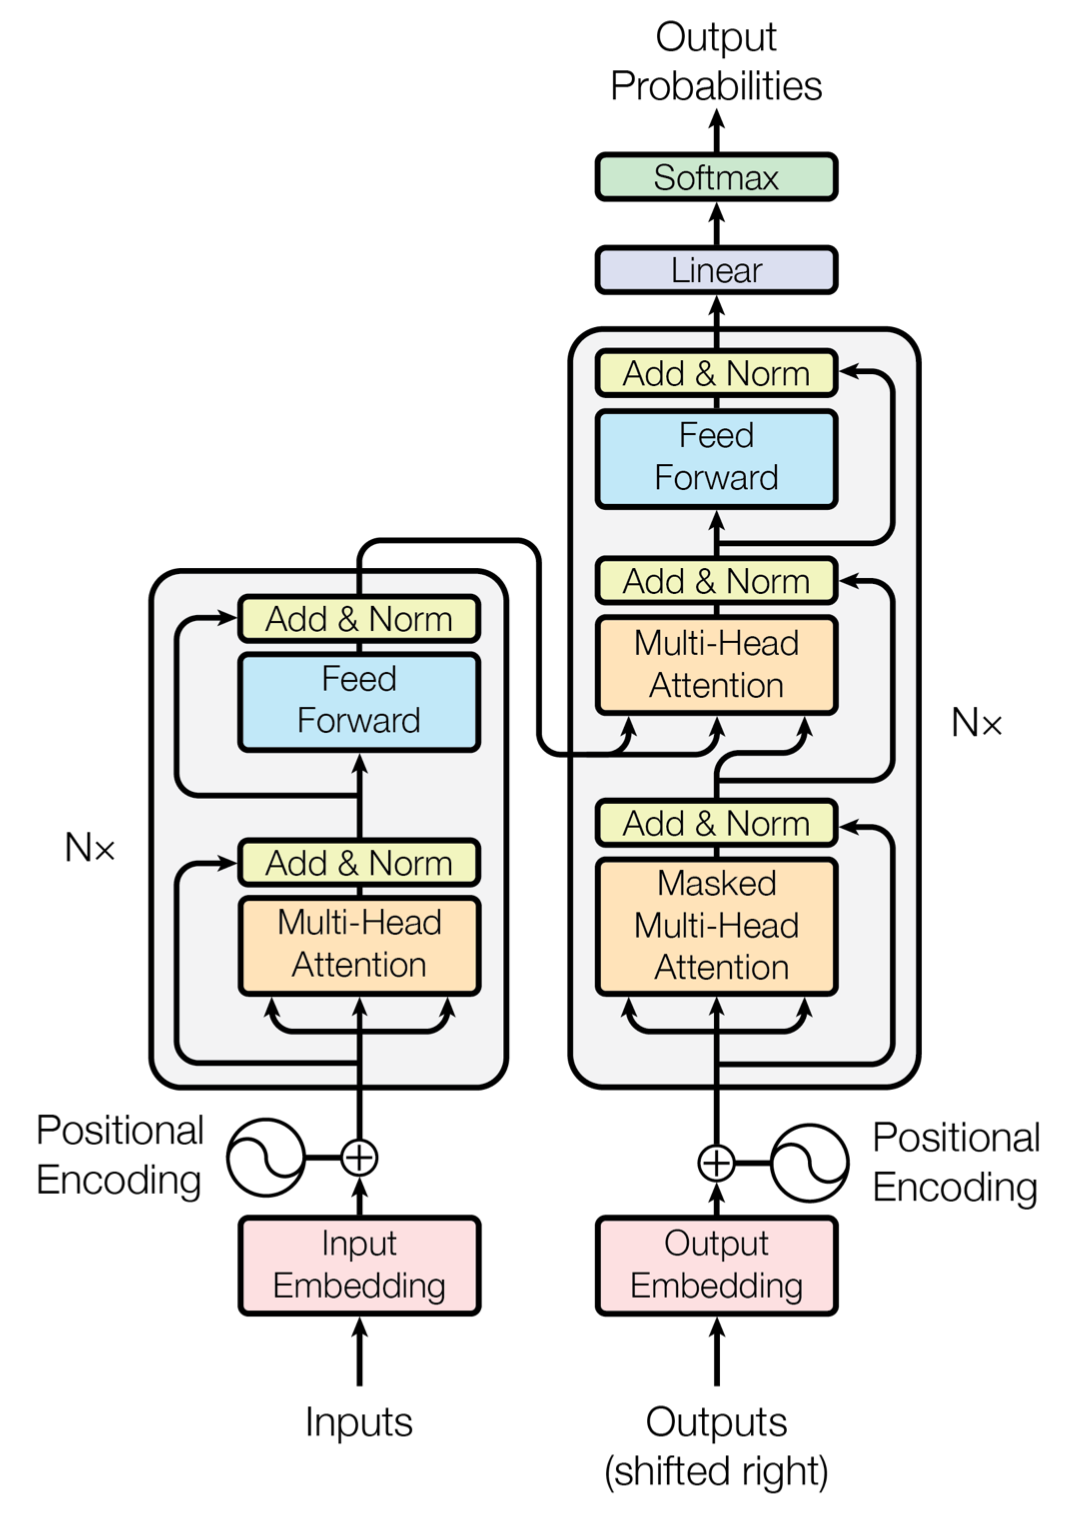
\includegraphics[width=0.8\linewidth, keepaspectratio]{images/architectures/t.png}
    
    \caption{The architecture introduced by Vaswani in the famous paper \textit{"Attention is All You Need"}~\cite{vaswani2017attention}.}
    \label{fig:uno}
\end{figure}

\section{Another Section in the Second Chapter}
Example of a table with its citation, Table~\ref{tab:table_example}.

\begin{table}[tb] % Start of floating table environment; [tb] = top or bottom of the page
\centering % Centers the table
\caption{Example of a table with various fields, checkmarks, and crosses.} % Caption
\begin{adjustbox}{width=0.9\textwidth} % Fits the table to 90% of the text width
{\normalsize % Sets normal font size
\setlength{\tabcolsep}{8pt} % Sets horizontal spacing between columns

\begin{tabular}{cccrrrr} % Creates a table with 7 columns:
                         % c = centered alignment, r = right alignment
\toprule % Thick upper horizontal rule (booktabs)

% \makecell allows formatted or multi-line text inside a cell.
% It is especially useful in headers to avoid using \parbox or \multicolumn.
% Here it is used to center and bold the header text.
\makecell[c]{\textbf{Fruit}} & 
\makecell[c]{\textbf{Orange-colored}} & 
\makecell[c]{\textbf{Peelable}} & 
\makecell[c]{\textbf{Weight}} &   
\makecell[c]{\textbf{Price}} &   
\makecell[c]{\textbf{Sugar}} &   
\makecell[c]{\textbf{Rating (1–10)}} \\  
% The symbol & separates columns within a row.
% Each cell of a row is delimited by an &.
% The \\ command ends the row and starts a new one.
\midrule % Medium horizontal rule

Orange & \checkmark  & \checkmark & 0.200 & 2.50 & 9.0 & 8 \\ % Example of a row: & separates columns, \\ closes the row
Mandarin & \checkmark & \checkmark & 0.120 & 3.20 & 8.5 & 9 \\
Lemon & \ding{55} & \checkmark & 0.100 & 3.50 & 2.5 & 6 \\
\midrule

Apple & \ding{55} & \ding{55} & 0.180 & 2.80 & 10.0 & 8 \\
Banana & \ding{55} & \checkmark & 0.150 & 1.10 & 12.2 & 9 \\
Kiwi & \ding{55} & \checkmark & 0.120 & 4.00 & 9.1 & 7 \\
Mango & \checkmark & \checkmark & 0.300 & 5.00 & 14.0 & 10 \\
\bottomrule % Thick lower horizontal rule

\end{tabular} % End of tabular environment
} % End of \normalsize block
\end{adjustbox} % End of width adjustment
\label{tab:table_example} % Label for referencing
\vspace{-10pt} % Reduces space below the table
\end{table} % End of table environment
 % input helps to keep the latex code cleaner by moving the table into another file

\section{Mathematical Formulas}
Here are two examples of how to write mathematical formulas. As you can easily recognize in Eq.~\ref{eq:continuous_ft}, we have the integral form of the Fourier Transform, while in Eq.~\ref{eq:discrete_ft} we see its discretized version using a summation.

% --- Formula 1: Continuous Fourier Transform (The Integral) ---
\begin{equation}
    \label{eq:continuous_ft}
    X(f) = \int_{-\infty}^{\infty} x(t) e^{-j 2\pi f t} \, dt
\end{equation}

% --- Formula 2: Discrete Fourier Transform (The Summation) ---
\begin{equation}
    \label{eq:discrete_ft}
    X_k = \sum_{n=0}^{N-1} x_n \cdot e^{-i \frac{2\pi}{N} k n}
\end{equation}

\section{Algorithm Example}
In Algorithm \ref{alg:dijkstra}, one way to compute the shortest path can be seen.

\begin{algorithm}[H] % H forces placement exactly here. Not recommended to always use it.
\caption{Dijkstra's Algorithm}
\label{alg:dijkstra}

    \begin{algorithmic}[1]
        
        \Procedure{Dijkstra}{$G, s$} 
            
            \State $dist[] \gets \infty$ \Comment{Initialize distances to infinity}
            \State $dist[s] \gets 0$     \Comment{Distance to the source is 0}
            \State $Q \gets V[G]$        \Comment{Add all nodes to the queue}
            
            \While{$Q$ is not empty} 
                \State $u \gets$ vertex in $Q$ with minimum $dist[u]$
                \State remove $u$ from $Q$
                
                \For{each neighbor $v$ of $u$} 
                    \State $alt \gets dist[u] + length(u, v)$
                    
                    \If{$alt < dist[v]$} 
                        \State $dist[v] \gets alt$
                        \State $prev[v] \gets u$
                    \EndIf
                    
                \EndFor
            \EndWhile
            
            \State \textbf{return} $dist[], prev[]$
            
        \EndProcedure 
        
    \end{algorithmic}
\end{algorithm}

\section{Code Examples}
You may also include some code samples, as long as they are not too long. An example can be seen in Code \ref{cod:hello}.

\begin{lstlisting}[caption={Example code, taken from helloworldspam.py}, label={cod:hello}]
print('Starting the ultimate hello world spammer')
for i in range(10000000):
    print("Hello, world!")
\end{lstlisting}

\section{Bibliography Management}
All bibliographic references must be inserted into the project’s ``.bib'' file. In this template, the file is ``bibliography.bib''. To cite a reference, use the command ``\textbackslash cite\{<id>\}'', such as \cite{vaswani2017attention}.
